\documentclass{beamer}

%
% Use Packages
%

\usepackage{hyperref}
%\usepackage[acronym,toc]{glossaries} %%%% Acronym/glossary support
\usepackage[]{glossaries-extra}
\glsenableentrycount
%\usepackage{authblk}
\usepackage [english]{babel}
\usepackage [autostyle, english = american]{csquotes}
\MakeOuterQuote{"}
\usepackage[flushleft]{threeparttable}
%\usepackage[margin=1.0in]{geometry}
%\usepackage[plain]{algorithm}
\usepackage{cite}
\usepackage{soul}
\usepackage{xspace}

\newcommand{\Cyclus}{\textsc{Cyclus}\xspace}
\newcommand{\Cycamore}{\textsc{Cycamore}\xspace}
\newcommand{\Trailmap}{\textsc{Trailmap}\xspace}

\author{Kathryn A. Mummah, Paul P.H. Wilson\\University of Wisconsin - Madison}

\setbeamertemplate{bibliography item}{\insertbiblabel}

\date{January, 2021} 
\title{The \Cyclus Fuel Cycle Simulator and Applications of \Cyclus for International Safeguards}

\AtBeginSection[]
{
    \begin{frame}
        \frametitle{Table of Contents}
        \tableofcontents[currentsection]
    \end{frame}
}

\usetheme[white,nav]{Wisconsin}
\begin{document}
\newcommand*{\alphabet}{ABCDEFGHIJKLMNOPQRSTUVWXYZabcdefghijklmnopqrstuvwxyz}
\newlength{\highlightheight}
\newlength{\highlightdepth}
\newlength{\highlightmargin}
\setlength{\highlightmargin}{2pt}
\settoheight{\highlightheight}{\alphabet}
\settodepth{\highlightdepth}{\alphabet}
\addtolength{\highlightheight}{\highlightmargin}
\addtolength{\highlightdepth}{\highlightmargin}
\addtolength{\highlightheight}{\highlightdepth}
\newcommand*{\Highlight}{\rlap{\textcolor{HighlightBackground}{\rule[-\highlightdepth]{\linewidth}{\highlightheight}}}}
  
\begin{frame}
\titlepage
\end{frame}

%% Slides

% \begin{frame}
% \frametitle{Outline}
% \tableofcontents
% \end{frame}

\section*{Outlines}
\frame{
\frametitle{Outline of Part I: Nuclear Fuel Cycle Simulators:\\What and Why}
\tableofcontents[part=1]}
%\subsection{Part II: Trailmap: Applying \Cyclus to International Safeguards}
\frame{
\frametitle{Outline of Part II: Trailmap: Applying \Cyclus\\to International Safeguards}
\tableofcontents[part=2]}

\part{Nuclear Fuel Cycle Simulators: What and Why}
\frame{\partpage}

\section{Fuel Cycle Simulators}
\subsection{What and Why?}
% ---------------------------------------------- %
% Fuel Cycle Simulators Track Flows of Nuclear Material
\begin{frame}{Fuel Cycle Simulators Track Flows of Nuclear Material}
\begin{columns}
    \column{0.45\textwidth}
    \begin{itemize}
        \item System-scale tool to model nuclear material flow between facilities
        \item Can be as simple as an Excel spreadsheet
        \item Most common usage is transition studies
        \item Should be able to inform non-technical as well as technical decision-makers
    \end{itemize}
    \column{0.55\textwidth}
        \begin{figure}[h]
            \centering
            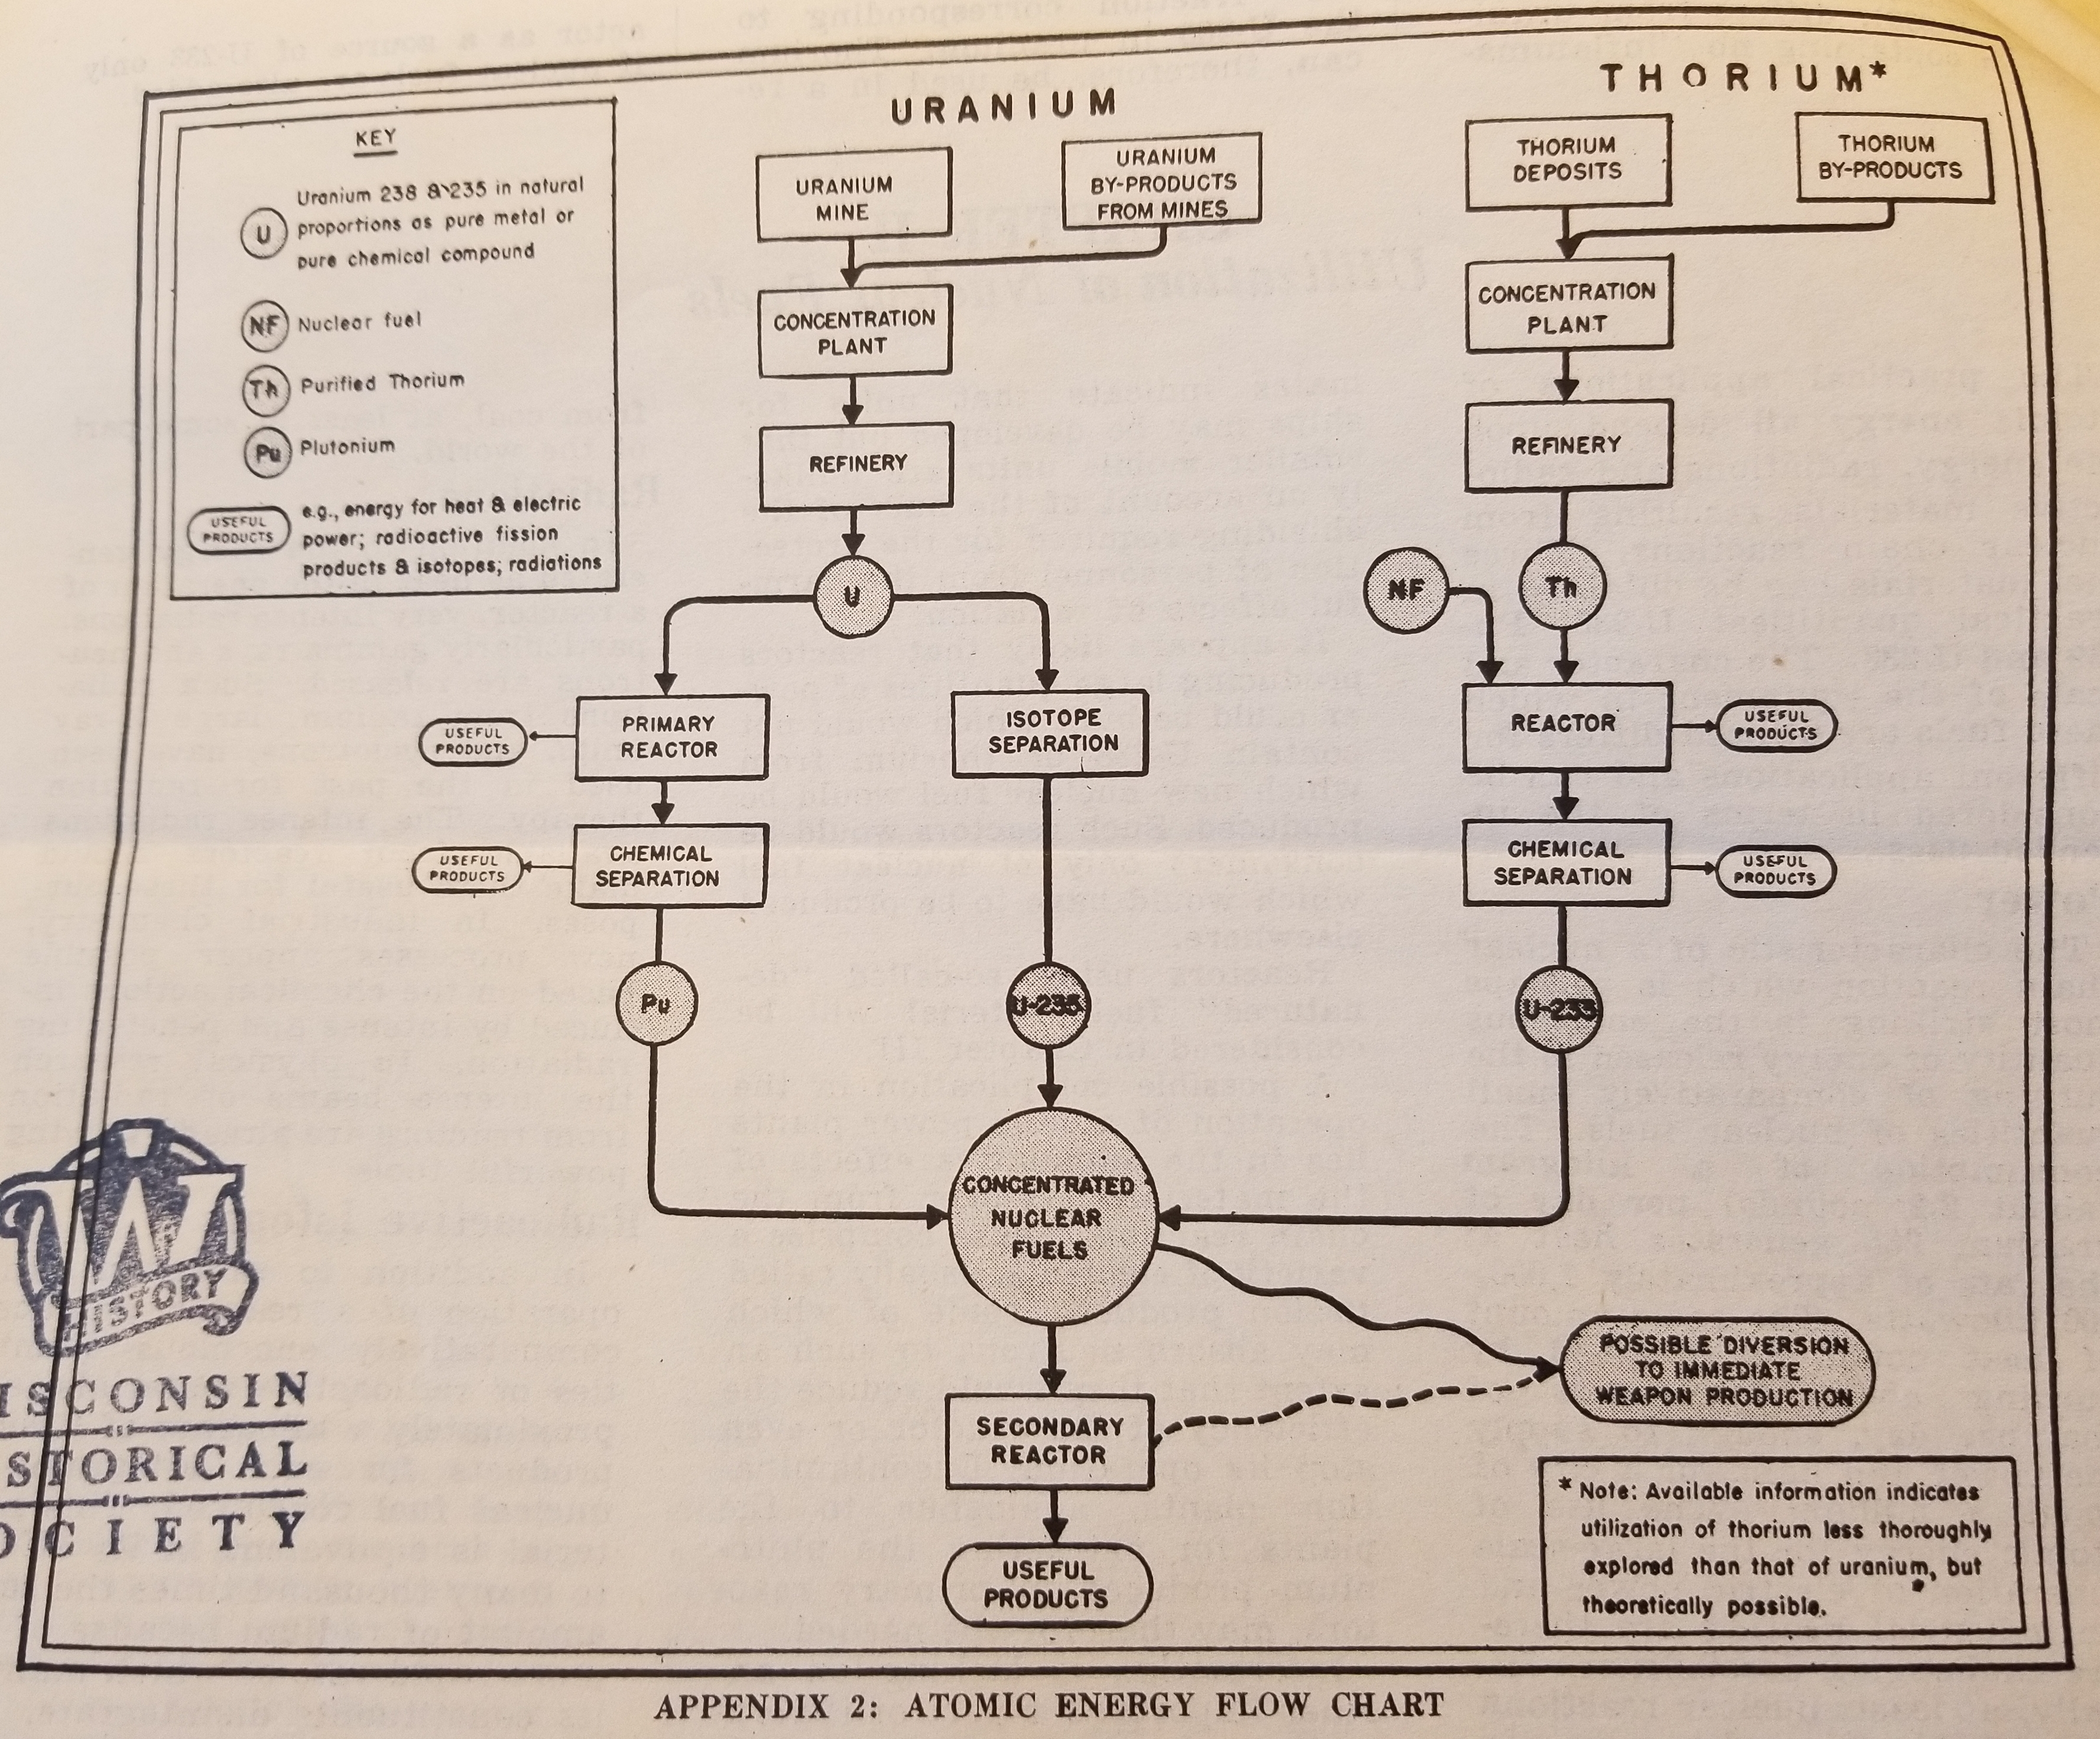
\includegraphics[width=\linewidth]{images/very-old-fuel-cycle1.jpg}
            \caption{U.N. Report, Scientific and Technical Aspects of the Control of Atomic Energy, 1946 \cite{noauthor_scientific_1946}}
            \label{fig:old-fc-diagram}
        \end{figure}
\end{columns}
\end{frame}
% ---------------------------------------------- %

% ---------------------------------------------- %
% Cyclus
\begin{frame}{Transition Studies Require Dynamic (Time-Dependent)\\Capabilities}
    \begin{figure}
        \centering
        \includegraphics[width=\linewidth]{images/Cyclus.png}
        \caption{Classic usage of a fuel cycle simulator includes designing a timeline of new facilities and retirements to transition to a new fuel cycle}
        \label{fig:ABR}
    \end{figure}
\end{frame}
% ---------------------------------------------- %


\subsection{Existing Fuel Cycle Simulators}
% ---------------------------------------------- %
% Cyclus
\begin{frame}{An Incomplete List of Fuel Cycle Simulators}
    \begin{table}[]
    \centering
    %\caption{Fuel Cycle Simulation Tools}
    \small
    \begin{tabular}{|p{2.4cm}|p{2.2cm}|p{2.cm}|p{1.cm}|p{1.3cm}|p{.7cm}|}
        \hline Tool & Developer & Access & Dynam/ \newline Static & Update? & First \newline Pub \\ \hline
        CAFCA \cite{guerin_impact_2009} & MIT & Licensed (f) & D &  Dormant & 2004 \\ %updated?? Discrete
        CLASS \cite{mouginot_core_2014} & France & Open-source & D & Yes & 2013 \\ %Core Library for Advanced Scenario Simulation, Discrete
        COSI \cite{meyer_new_2009},\cite{boucher_cosi:_2006} & CEA & Proprietary & D & Yes & 1991 \\
        \Cyclus \cite{huff_fundamental_2016} & UW--Madison & Open-source & D & Yes & 2011\\ %Discrete
        DANESS \cite{van_den_durpel_daness_2003} & Nuclear21 & Proprietary & D &Yes & 2003 \\
        DESAE \cite{andrianova_desae_2008} & IAEA INPRO & Unknown & D & D & 2006 \\
        DYMOND \cite{moisseytsev_dymond_2001} & ANL & Proprietary & D & Yes &2001 \\
        FUTURE \cite{kim_development_2013} & Korea & Unknown & D & Yes & 2013 \\
        MAKAL \cite{shay_epa_2006} & IEA & Proprietary & D & Yes & 1970s \\
        NFCSim \cite{schneider_nfcsim:_2005} & LANL & Proprietary & D &  No & 2005 \\ %discrete
        NFCSS \cite{noauthor_nuclear_2007} & IAEA & Open GUI & S & Yes & 1996 \\ %Fleet-based
        ORION \cite {worrall_scenario_2007} & ORNL/UKNNL & Proprietary & D & Yes & 2007 \\ %Discrete
        ROADMAP\cite{noauthor_iaea_2018} & IAEA & Unknown & U &  Yes & 2018 \\ %discrete unknown
        SITON \cite{brolly_physical_2017} & Hungary & Unknown & D & Yes & 2017\\ %Discrete
        VISION \cite{jacobson_vision_2009} & INL & Licensed (f) & D & Yes & 2006 \\
        VEGAS \cite{schneider_vegas:_2016} & UT--Austin & Licensed (f) & D & Uknown & 2017 \\   \hline %preconditioner Fleet-based
    \end{tabular}
    \label{tab:FCS}
\end{table}
\end{frame}
% ---------------------------------------------- %

\subsection{Why did UW--Madison create a fuel cycle simulator?}
% ---------------------------------------------- %
% Why another fuel cycle simulator?
\begin{frame}{Why another fuel cycle simulator?}
\begin{columns}
    \column{0.55\textwidth}
    Gaps were noted in fuel cycle simulation capabilities during the Global Nuclear Energy Partnership (GNEP) push of the late 2000s
    \begin{itemize}
        \item Proprietary tools
        \item Mostly focused on reactor simulations
        \item Limited or on ability to novel designs
        \item Static systems
    \end{itemize}
    \column{0.35\textwidth}
    \begin{block}{GNEP in a few words}
        \footnotesize
        \alert{GNEP} began in 2006 as a US-lead effort to expand nuclear energy domestically \& internationally to:
        \begin{itemize}
            \item Reduce usage on fossil fuels/promote clean energy
            \item Encourage proliferation- resistant designs
            \item Assert US dominance as global supplier
        \end{itemize}
        US effort killed by Obama admin amid the Great Recession, international effort replaced by IFNEC
    \end{block}
\end{columns}
\end{frame}
% ---------------------------------------------- %

\section{\Cyclus}
\subsection{Ethos of \Cyclus}
% ---------------------------------------------- %
% Cyclus
\begin{frame}{History and Goals of \Cyclus}
\begin{itemize}
    \item Successor to Global Evaluation of Nuclear Infrastructure Utilization Scenarios (GENIUS) tools
\end{itemize}

\alert{Goal: Flexibility}

\begin{itemize}
    \item Model innovative/unconventional technologies
    \item Minimal inherent technology assumptions
\end{itemize}

\alert{Goal: Modeling}

\begin{itemize}
    \item Discrete facilities with discrete material tracking
    \item Optimization and sensitivity analysis
\end{itemize}

\alert{Goal: Software}


\begin{itemize}
    \item Low barrier to adoption with rapid payback\footnote{The goal we're probably furthest from at this moment}
    \item Commonly and freely available software infrastructure, can run on all operating systems
\end{itemize}
\end{frame}
% ---------------------------------------------- %



\subsection{Agent-based modeling}
% ---------------------------------------------- %
% Cyclus
\begin{frame}{\Cyclus Overview\cite{huff_fundamental_2016}}

\begin{columns}
\column{0.5\textwidth}
\begin{figure}
    \centering
    \includegraphics[width=0.4\textwidth]{images/logo2.png}
    \label{fig:my_label}
\end{figure}
\begin{itemize}
    \item Open source modular fuel cycle simulator
    \item Market-based exchange of resources (commodities)
    \item Discrete facilities (even when identical)
    \item Discrete material tracking at the nuclide level
    \item Time-dependent
    \item Parallelizable
\end{itemize}
\column{0.5\textwidth}
\begin{figure}
    \centering
    \includegraphics[width=0.9\textwidth]{images/cyclus_region_inst_facility.jpg}
    \caption{From \textit{Fundamental concepts in the Cyclus nuclear fuel cycle simulation framework} by Huff \textit{et al.}\cite{huff_fundamental_2016}}
    \label{fig:Cyclus_setup}
\end{figure}
\end{columns}

\end{frame}
% ---------------------------------------------- %


% ---------------------------------------------- %
\begin{frame}{Agent-based model}
\begin{columns}
\column{0.45\textwidth}
\begin{itemize}
    \item \Cyclus coordinates and tracks the \textbf{deployment of facilities} and \textbf{movement of materials between facilities}
    \item Facility models are "plug and play" through the API
    \item Allow for easy switch between lower and higher fidelity
    \item Similar to MOOSE framework collaboration
\end{itemize}
\column{0.5\textwidth}
\begin{figure}
    \centering
    \includegraphics[width=0.85\textwidth]{images/Cyclus_ecosystem.png}
    \caption{\Cyclus architecture encourages open collaboration while allowing closed development and users with sensitive information, image from \cite{huff_fundamental_2016}}
    \label{fig:cyclus_ecosystem}
\end{figure}
\end{columns}
\end{frame}
% ---------------------------------------------- %



% ---------------------------------------------- %
\begin{frame}{\Cyclus facility models}
\begin{columns}
\column{0.45\textwidth}
\begin{itemize}
    %\item \Cyclus Kernel only requires the ability to place and respond to bids (trade)
    \item \Cycamore includes simple models of common fuel cycle facilities
    \item Developers have contributed higher fidelity models such as 
    \begin{itemize}
        \item cyborg (Univ. of Tennessee)
        \item mbmore (Univ. of Wisconsin)
    \end{itemize}
    \item Anyone can develop an archetype
    \begin{itemize}
        \item Open and closed contributors, models (archetypes), and users
    \end{itemize}
\end{itemize}
\column{0.5\textwidth}
\begin{figure}
    \centering
    \includegraphics[width=0.85\textwidth]{images/Cyclus_ecosystem.png}
    \caption{\Cyclus architecture encourages open collaboration while allowing closed development and users with sensitive information, image from \cite{huff_fundamental_2016}}
    \label{fig:cyclus_ecosystem}
\end{figure}
\end{columns}
\end{frame}
% ---------------------------------------------- %


\subsection{Market Exchange of Commodities}
% ---------------------------------------------- %
\begin{frame}{Dynamic Resource Exchange}
\begin{itemize}
    \item At every timestep, \Cyclus gathers information about commodity requests
    \begin{itemize}
        \item Quantity
        \item Quality (isotopics)
        \item Can be XOR, such as MOX or UOX
    \end{itemize}
    \item \Cyclus then gathers bids and solves the flow graph
    \item Materials are transferred and the simulation moves forward to the next timestep
    \item Market-based exchange of resources (commodities)
    \begin{itemize}
        \item Nuclear materials
        \item Knowledge, design information, experts
        \item Economic units, money
    \end{itemize}
\end{itemize}
\end{frame}
% ---------------------------------------------- %

% ---------------------------------------------- %
\begin{frame}{Regions and Institutions}
    \begin{itemize}
        \item Reflects the geopolitical realities of nuclear facilities 
        \item Hierarchy is Region, Institution, Facility
        \item Region: State, could also be a geographical region smaller (e.g. the Midwest), or larger (e.g. Scandinavia) than a State 
        \item Institution: utility or government
        \item Institutions deploy facilities
        \item Flow can be prioritized within institution/region
        \item Institutions can reject material outside desired characteristics (e.g. above 5\% enriched) from other institutions
        \item Can be ignored (set to Null) if not relevant for a given simulation
    \end{itemize}
\end{frame}
% ---------------------------------------------- %


\subsection{\Cyclus Community}
% ---------------------------------------------- %
\begin{frame}{\Cyclus Community}
    \begin{columns}
    \column{0.9\textwidth}
    \begin{figure}
        \centering
        \includegraphics[width=\textwidth]{images/heat.png}
        \caption{Community is mainly university, national lab}
        \label{fig:my_label}
    \end{figure}
    \end{columns}
\end{frame}
% ---------------------------------------------- %

% ---------------------------------------------- %
\begin{frame}{\Cyclus Funders}
    \begin{columns}
    \column{0.6\textwidth}
    \begin{figure}
        \centering
        \includegraphics[width=\textwidth]{images/Cyclus-funders.png}
        %\caption{}
        \label{fig:my_label}
    \end{figure}
    \column{0.3\textwidth}
    Diverse albeit intermittent funding sources over the last decade
    \end{columns}
\end{frame}
% ---------------------------------------------- %

\part{Trailmap: Applying \Cyclus to International Safeguards}
\frame{\partpage}


\section{Directed graph fuel cycle analysis and \Cyclus}
\subsection{Acquisition Pathway Analysis (APA)}

\begin{frame}{Motivation}
\begin{block}{Acquisition Pathway Analysis (APA)} Assess technically plausible steps a State could take to acquire material that could be used in a nuclear explosive device \cite{amano_conceptualization_2013}
\end{block}
  \begin{itemize}
  \medskip
  %\item Enhance state evaluation capabilities (IAEA R\&D objective V.2.R1)
    \item Objective and reproducible analysis for any set of fuel cycle facilities and capabilities
  \item Bring experience in modeling nuclear material flows to the nonproliferation and safeguards community
    \bigskip
    \begin{figure}
        \centering
        \includegraphics[width=0.95\linewidth]{images/path_step_types.png}
        \caption{Four path steps to capture, based on \cite{renis_conducting_2014}}
        \label{fig:path_steps}
    \end{figure}

  \end{itemize}

\end{frame}


\subsection{\Trailmap}
% ---------------------------------------------- %
\begin{frame}{Introducing \Trailmap}
    \begin{columns}
     \column{0.55\textwidth}
     \begin{itemize}
         \item \Trailmap is a new Cyclus module to conduct APA
     \end{itemize}
     \bigskip
    Before running \Trailmap
    \begin{itemize}
        \item User gathers State-specific factors and information
        \item Creates a \Cyclus input file with the set of existing facilities as well as technologically feasible undeclared activities and facilities
    \end{itemize}
    \column{0.45\textwidth}
    \begin{figure}
        \centering
        \includegraphics[width=0.85\textwidth]{images/Trailmap.png}
        \caption{From MTB Project}
        \label{fig:mtb}
    \end{figure}
    \end{columns}
    \bigskip
   Trailmap is also open-source and is available at \href{https://github.com/cnerg/trailmap}{https://github.com/cnerg/trailmap}
\end{frame}
% ---------------------------------------------- %

% ---------------------------------------------- %
\begin{frame}{\Trailmap}

    \begin{enumerate}
        \item Identify installed \Cyclus modules
        \item Reads in \Cyclus input file, identifying agents and commodities
        \item Builds a directed graph $G = (V, \ E)$ of facilities and commodities using NetworkX
        \item Depth-first search from all sources to all sinks
        \item Visualize graph using Jupyter notebook
        \item Filter and sort pathways using analysis tools
        \item Run Cyclus for individual path or groups of paths
    \end{enumerate}
    \color{gray}{\small{Future work}}
    \begin{enumerate}
        \setcounter{enumi}{6}
        {\setbeamercolor{enumerate item}{fg=gray}\color{gray}
        \item Further sorting and filtering of pathways based on throughput
        \item Test notional safeguards}
    \end{enumerate}
\end{frame}
% ---------------------------------------------- %


\subsection{\Trailmap Demonstration}
% ---------------------------------------------- %
\begin{frame}{Example "Republic of Bundy"}
    \begin{columns}
    \column{0.53\textwidth}
    \begin{figure}
        \centering
        \includegraphics[width=\textwidth]{images/example.png}
        \caption{Network flow of "ROB" fuel cycle}
        \label{fig:ROB}
    \end{figure}
    \column{0.42\textwidth}
    \begin{itemize}
        \item Small but well-developed fuel cycle
        \item Civilian declared enrichment and reprocessing
        \item Clandestine enrichment facility
    \end{itemize}
    \begin{figure}[h]
        \centering
        \includegraphics[width=0.8\linewidth]{images/Bundy.jpg}
        \caption{\small Former foster dog Bundy}
        \label{fig:my_label}
    \end{figure}
    \end{columns}
\end{frame}
% ---------------------------------------------- %

% ---------------------------------------------- %
\begin{frame}{Pathways}
    \begin{itemize}
        \item Mine, Mill, Conversion, Declared Enrichment, Tails
        \item Mine, Mill, Conversion, Undeclared Enrichment, HEU/Pu
        \item Mine, Mill, Conversion, Declared Enrichment, Fuel Fab, LWR, Waste Storage, Reprocessing, MOX Fuel Fab, HEU/Pu
        \item Mine, Mill, Conversion, Declared Enrichment, Fuel Fab, LWR, Reprocessing, MOX Fuel Fab, HEU/Pu
        \item Mine, Mill, Conversion, Declared Enrichment, Fuel Fab, LWR, Reprocessing, HEU/Pu
        \item Mine, Mill, Conversion, Declared Enrichment, Undeclared Enrichment, HEU/Pu
        \item Mine, Mill, Conversion, Declared Enrichment, Fuel Fab, LWR, Waste Storage, Reprocessing, HEU/Pu
        \item Mine, Mill, Conversion, Declared Enrichment, HEU/Pu
        \item Mine, Mill, Conversion' Declared Enrichment, Undeclared Enrichment, Undeclared Tails,
        \item Mine, Mill, Conversion, Declared Enrichment, Undeclared Tails
    \end{itemize}
\end{frame}
% ---------------------------------------------- %

% ---------------------------------------------- %
\begin{frame}{Acquisition Paths}
    \begin{itemize}
        \item \st{Mine, Mill, Conversion, Declared Enrichment, Tails}
        \item Mine, Mill, Conversion, Undeclared Enrichment, HEU/Pu
        \item Mine, Mill, Conversion, Declared Enrichment, Fuel Fab, LWR, Waste Storage, Reprocessing, MOX Fuel Fab, HEU/Pu
        \item Mine, Mill, Conversion, Declared Enrichment, Fuel Fab, LWR, Reprocessing, MOX Fuel Fab, HEU/Pu
        \item Mine, Mill, Conversion, Declared Enrichment, Fuel Fab, LWR, Reprocessing, HEU/Pu
        \item Mine, Mill, Conversion, Declared Enrichment, Undeclared Enrichment, HEU/Pu
        \item Mine, Mill, Conversion, Declared Enrichment, Fuel Fab, LWR, Waste Storage, Reprocessing, HEU/Pu
        \item Mine, Mill, Conversion, Declared Enrichment, HEU/Pu
        \item \st{Mine, Mill, Conversion' Declared Enrichment, Undeclared Enrichment, Undeclared Tails}
        \item \st{Mine, Mill, Conversion, Declared Enrichment, Undeclared Tails}
    \end{itemize}
\end{frame}
% ---------------------------------------------- %


% ---------------------------------------------- %
\begin{frame}{Visualizing}
    \begin{itemize}
        \item Automated interactive visualization using Jupyter Notebooks and Plotly package
        \item Graphviz 'dot' to layout nodes
        \begin{itemize}
            \item Good starting point, designed for trees
            \item NFC are not quite trees, but almost
        \end{itemize}
    \end{itemize}
    \begin{figure}
        \centering
        \includegraphics[width=0.75\textwidth]{images/newplot.png}
        \label{fig:example_viz}
    \end{figure}
\end{frame}
% ---------------------------------------------- %


% ---------------------------------------------- %
\begin{frame}{Facility-specific pathways: reprocessing}
    \begin{itemize}
        \item \st{Mine, Mill, Conversion, Declared Enrichment, Tails}
        \item Mine, Mill, Conversion, Undeclared Enrichment, HEU/Pu
        \item \textbf{Mine, Mill, Conversion, Declared Enrichment, Fuel Fab, LWR, Waste Storage, Reprocessing, MOX Fuel Fab, HEU/Pu}
        \item \textbf{Mine, Mill, Conversion, Declared Enrichment, Fuel Fab, LWR, Reprocessing, MOX Fuel Fab, HEU/Pu}
        \item \textbf{Mine, Mill, Conversion, Declared Enrichment, Fuel Fab, LWR, Reprocessing, HEU/Pu}
        \item Mine, Mill, Conversion, Declared Enrichment, Undeclared Enrichment, HEU/Pu
        \item \textbf{Mine, Mill, Conversion, Declared Enrichment, Fuel Fab, LWR, Waste Storage, Reprocessing, HEU/Pu}
        \item Mine, Mill, Conversion, Declared Enrichment, HEU/Pu
        \item \st{Mine, Mill, Conversion' Declared Enrichment, Undeclared Enrichment, Undeclared Tails}
        \item \st{Mine, Mill, Conversion, Declared Enrichment, Undeclared Tails}
    \end{itemize}
\end{frame}
% ---------------------------------------------- %

% ---------------------------------------------- %
\begin{frame}{Shortest pathways}
    \begin{itemize}
        \item \st{Mine, Mill, Conversion, Declared Enrichment, Tails}
        \item \textcolor{red}{Mine, Mill, Conversion, Undeclared Enrichment, HEU/Pu}
        \item Mine, Mill, Conversion, Declared Enrichment, Fuel Fab, LWR, Waste Storage, Reprocessing, MOX Fuel Fab, HEU/Pu
        \item Mine, Mill, Conversion, Declared Enrichment, Fuel Fab, LWR, Reprocessing, MOX Fuel Fab, HEU/Pu
        \item Mine, Mill, Conversion, Declared Enrichment, Fuel Fab, LWR, Reprocessing, HEU/Pu
        \item Mine, Mill, Conversion, Declared Enrichment, Undeclared Enrichment, HEU/Pu
        \item Mine, Mill, Conversion, Declared Enrichment, Fuel Fab, LWR, Waste Storage, Reprocessing, HEU/Pu
        \item \textcolor{red}{Mine, Mill, Conversion, Declared Enrichment, HEU/Pu}
        \item \st{Mine, Mill, Conversion' Declared Enrichment, Undeclared Enrichment, Undeclared Tails}
        \item \st{Mine, Mill, Conversion, Declared Enrichment, Undeclared Tails}
    \end{itemize}
\end{frame}
% ---------------------------------------------- %


% ---------------------------------------------- %
\begin{frame}{Other Tools}
    \begin{itemize}
        \item Search over a given list of facilities
        \begin{itemize}
            \item Pathways that contain \textit{any} facilities in the list
            \item Pathways that contain \textit{all} facilities in the list
        \end{itemize}
        \item Pathways that flow between a specific source and/or target node        \begin{itemize}
            \item Node disjoint paths
        \end{itemize}
        \item Cyclical or looping pathways (reprocessing)
        \item Graph parameters
        \begin{itemize}
            \item Graph semiconnectedness
            \item Flow hierarchy
            \item Shortest, longest paths
        \end{itemize}
        \item Flow (throughput)
        \begin{itemize}
            \item Flow of a given pathway
            \item Maximum total flow (complete breakout)
            \item Maximum flow pathway
            \item All pathways with flow above a threshold
        \end{itemize}
    \end{itemize}
\end{frame}
% ---------------------------------------------- %

\section{Conclusions \& Future Work}
% ---------------------------------------------- %
\begin{frame}{Conclusions}
    \begin{itemize}
        \item \Trailmap can conduct APA
        \item Basic interactive visualization is running
        \item \Trailmap is mostly a command-line tool right now, but can also be used from a Jupyter Notebook
        \item Next up: 
        \begin{itemize}
            \item Automating import of throughput information from \Cyclus simulation into \Trailmap
            \item Calculating time to completion for paths of interest
            \item Revamp visualization tool
        \end{itemize}
    \end{itemize}
\end{frame}
% ---------------------------------------------- %

% ---------------------------------------------- %
\begin{frame}{Future Work}
    \begin{itemize}
        \item Capture time-dependent evolution of acquisition paths
        \item Evaluate user interface to \Trailmap
        \item Add MBAs to existing \Cyclus facilities and build notional safeguards
        \begin{itemize}
            \item Expand MBAs and signatures from recycle:Pyre archetype \cite{westphal_modeling_2019}
            \item Expand inspector swipes from mbmore:RandomEnrich\cite{mcgarry_mbmore_2018}
        \end{itemize}
    \end{itemize}
    \begin{figure}
        \centering
        \includegraphics[width=0.3\textwidth]{images/Mcgarry_diversion.png}
        \caption{mbmore modeling of protracted diversion at an enrichment facility}
        \label{fig:McGarry_diversion}
    \end{figure}
\end{frame}
% ---------------------------------------------- %


\begin{frame}{Funding}
    \begin{itemize}
        \item This research was performed under appointment to the Nuclear Nonproliferation International Safeguards Fellowship Program sponsored by the National Nuclear Security Administration’s Office of International Nuclear Safeguards (NA-241)
        \item This work was funded in-part by the Consortium for Verification Technology under Department of Energy National Nuclear Security Administration award number DE-NA0002534.
        \item I gratefully acknowledge the support of the U.S. Department of Energy through the 
        \begin{itemize}
            \item LANL/LDRD Program
            \item G. T. Seaborg Institute
            \item Nuclear Criticality Safety Program
        \end{itemize} for this work.
    \end{itemize}

\end{frame}

\begin{frame}[allowframebreaks]{References}
    \bibliographystyle{ans}
{\footnotesize\bibliography{references}}
\end{frame}

\end{document}